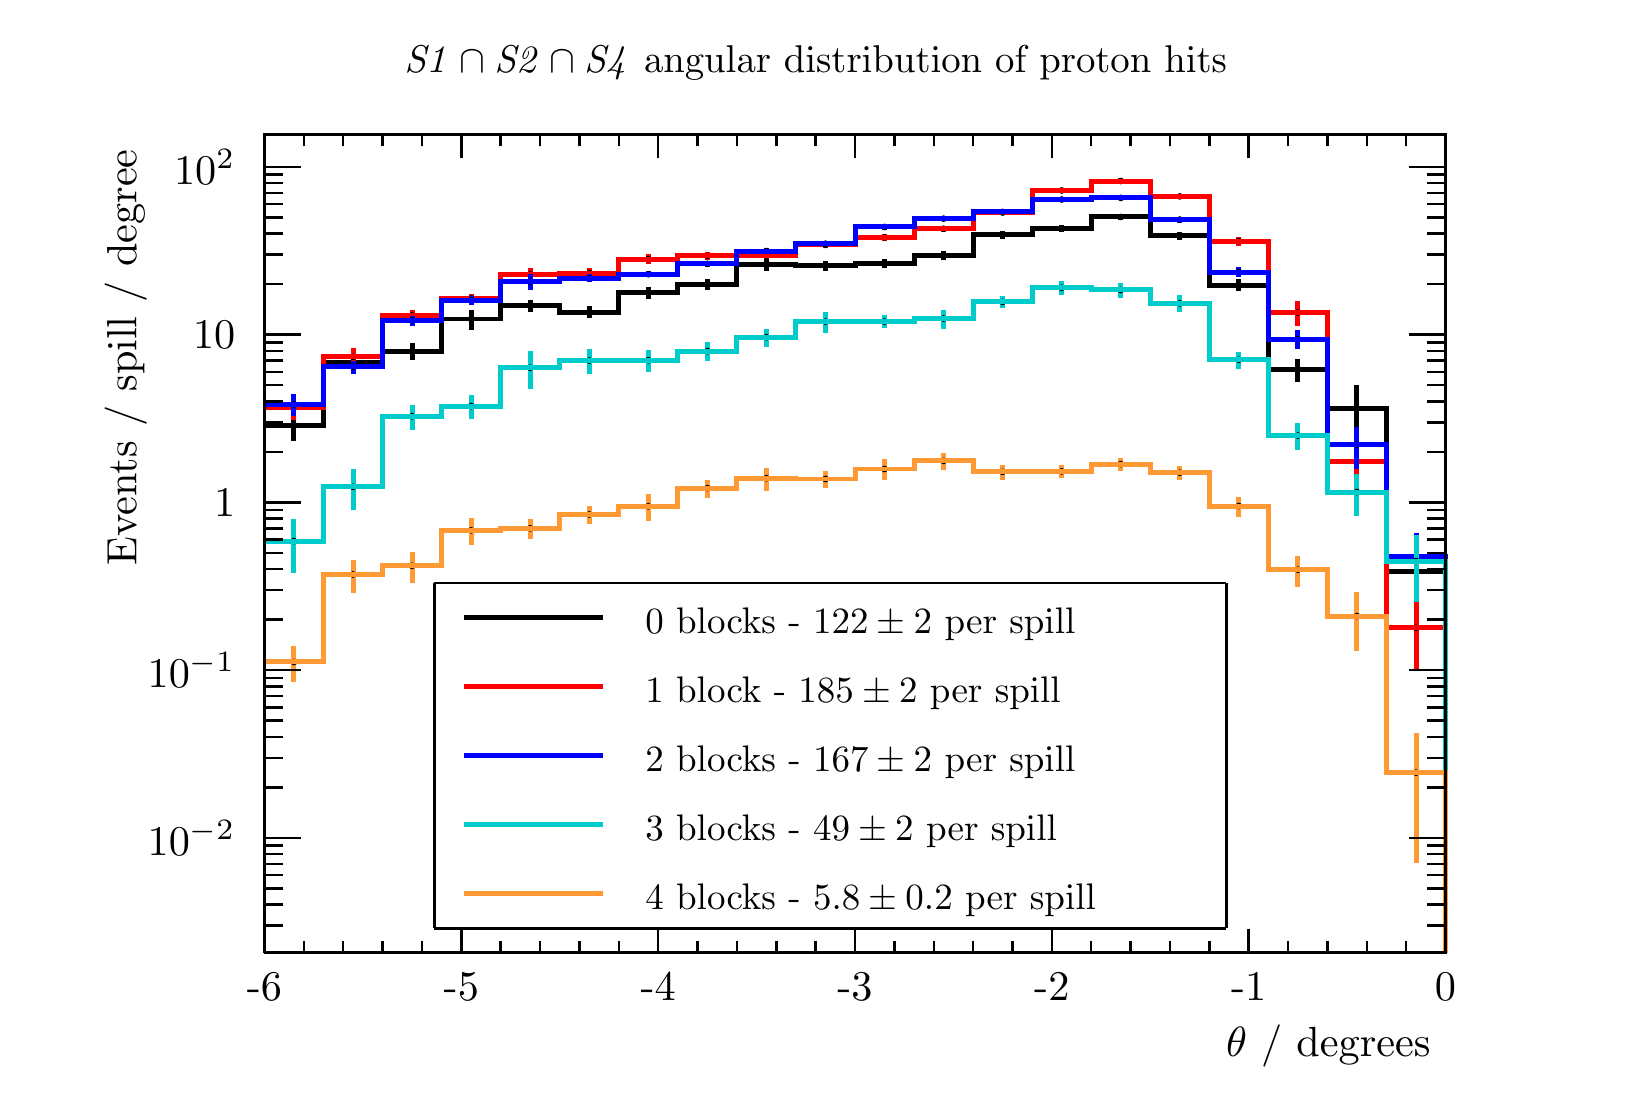
\begin{tikzpicture}
\pgfdeclareplotmark{cross} {
\pgfpathmoveto{\pgfpoint{-0.3\pgfplotmarksize}{\pgfplotmarksize}}
\pgfpathlineto{\pgfpoint{+0.3\pgfplotmarksize}{\pgfplotmarksize}}
\pgfpathlineto{\pgfpoint{+0.3\pgfplotmarksize}{0.3\pgfplotmarksize}}
\pgfpathlineto{\pgfpoint{+1\pgfplotmarksize}{0.3\pgfplotmarksize}}
\pgfpathlineto{\pgfpoint{+1\pgfplotmarksize}{-0.3\pgfplotmarksize}}
\pgfpathlineto{\pgfpoint{+0.3\pgfplotmarksize}{-0.3\pgfplotmarksize}}
\pgfpathlineto{\pgfpoint{+0.3\pgfplotmarksize}{-1.\pgfplotmarksize}}
\pgfpathlineto{\pgfpoint{-0.3\pgfplotmarksize}{-1.\pgfplotmarksize}}
\pgfpathlineto{\pgfpoint{-0.3\pgfplotmarksize}{-0.3\pgfplotmarksize}}
\pgfpathlineto{\pgfpoint{-1.\pgfplotmarksize}{-0.3\pgfplotmarksize}}
\pgfpathlineto{\pgfpoint{-1.\pgfplotmarksize}{0.3\pgfplotmarksize}}
\pgfpathlineto{\pgfpoint{-0.3\pgfplotmarksize}{0.3\pgfplotmarksize}}
\pgfpathclose
\pgfusepathqstroke
}
\pgfdeclareplotmark{cross*} {
\pgfpathmoveto{\pgfpoint{-0.3\pgfplotmarksize}{\pgfplotmarksize}}
\pgfpathlineto{\pgfpoint{+0.3\pgfplotmarksize}{\pgfplotmarksize}}
\pgfpathlineto{\pgfpoint{+0.3\pgfplotmarksize}{0.3\pgfplotmarksize}}
\pgfpathlineto{\pgfpoint{+1\pgfplotmarksize}{0.3\pgfplotmarksize}}
\pgfpathlineto{\pgfpoint{+1\pgfplotmarksize}{-0.3\pgfplotmarksize}}
\pgfpathlineto{\pgfpoint{+0.3\pgfplotmarksize}{-0.3\pgfplotmarksize}}
\pgfpathlineto{\pgfpoint{+0.3\pgfplotmarksize}{-1.\pgfplotmarksize}}
\pgfpathlineto{\pgfpoint{-0.3\pgfplotmarksize}{-1.\pgfplotmarksize}}
\pgfpathlineto{\pgfpoint{-0.3\pgfplotmarksize}{-0.3\pgfplotmarksize}}
\pgfpathlineto{\pgfpoint{-1.\pgfplotmarksize}{-0.3\pgfplotmarksize}}
\pgfpathlineto{\pgfpoint{-1.\pgfplotmarksize}{0.3\pgfplotmarksize}}
\pgfpathlineto{\pgfpoint{-0.3\pgfplotmarksize}{0.3\pgfplotmarksize}}
\pgfpathclose
\pgfusepathqfillstroke
}
\pgfdeclareplotmark{newstar} {
\pgfpathmoveto{\pgfqpoint{0pt}{\pgfplotmarksize}}
\pgfpathlineto{\pgfqpointpolar{44}{0.5\pgfplotmarksize}}
\pgfpathlineto{\pgfqpointpolar{18}{\pgfplotmarksize}}
\pgfpathlineto{\pgfqpointpolar{-20}{0.5\pgfplotmarksize}}
\pgfpathlineto{\pgfqpointpolar{-54}{\pgfplotmarksize}}
\pgfpathlineto{\pgfqpointpolar{-90}{0.5\pgfplotmarksize}}
\pgfpathlineto{\pgfqpointpolar{234}{\pgfplotmarksize}}
\pgfpathlineto{\pgfqpointpolar{198}{0.5\pgfplotmarksize}}
\pgfpathlineto{\pgfqpointpolar{162}{\pgfplotmarksize}}
\pgfpathlineto{\pgfqpointpolar{134}{0.5\pgfplotmarksize}}
\pgfpathclose
\pgfusepathqstroke
}
\pgfdeclareplotmark{newstar*} {
\pgfpathmoveto{\pgfqpoint{0pt}{\pgfplotmarksize}}
\pgfpathlineto{\pgfqpointpolar{44}{0.5\pgfplotmarksize}}
\pgfpathlineto{\pgfqpointpolar{18}{\pgfplotmarksize}}
\pgfpathlineto{\pgfqpointpolar{-20}{0.5\pgfplotmarksize}}
\pgfpathlineto{\pgfqpointpolar{-54}{\pgfplotmarksize}}
\pgfpathlineto{\pgfqpointpolar{-90}{0.5\pgfplotmarksize}}
\pgfpathlineto{\pgfqpointpolar{234}{\pgfplotmarksize}}
\pgfpathlineto{\pgfqpointpolar{198}{0.5\pgfplotmarksize}}
\pgfpathlineto{\pgfqpointpolar{162}{\pgfplotmarksize}}
\pgfpathlineto{\pgfqpointpolar{134}{0.5\pgfplotmarksize}}
\pgfpathclose
\pgfusepathqfillstroke
}
\definecolor{c}{rgb}{1,1,1};
\draw [color=c, fill=c] (0,0) rectangle (20,13.4957);
\draw [color=c, fill=c] (3,1.75444) rectangle (18,12.1461);
\definecolor{c}{rgb}{0,0,0};
\draw [c,line width=0.9] (3,1.75444) -- (3,12.1461) -- (18,12.1461) -- (18,1.75444) -- (3,1.75444);
\definecolor{c}{rgb}{1,1,1};
\draw [color=c, fill=c] (3,1.75444) rectangle (18,12.1461);
\definecolor{c}{rgb}{0,0,0};
\draw [c,line width=0.9] (3,1.75444) -- (3,12.1461) -- (18,12.1461) -- (18,1.75444) -- (3,1.75444);
\draw [c,line width=0.9] (3,1.75444) -- (3.75,1.75444) -- (3.75,1.75444) -- (4.5,1.75444) -- (4.5,1.75444) -- (5.25,1.75444) -- (5.25,1.75444) -- (6,1.75444) -- (6,1.75444) -- (6.75,1.75444) -- (6.75,1.75444) -- (7.5,1.75444) -- (7.5,1.75444) --
 (8.25,1.75444) -- (8.25,1.75444) -- (9,1.75444) -- (9,1.75444) -- (9.75,1.75444) -- (9.75,1.75444) -- (10.5,1.75444) -- (10.5,1.75444) -- (11.25,1.75444) -- (11.25,1.75444) -- (12,1.75444) -- (12,1.75444) -- (12.75,1.75444) -- (12.75,1.75444) --
 (13.5,1.75444) -- (13.5,1.75444) -- (14.25,1.75444) -- (14.25,1.75444) -- (15,1.75444) -- (15,1.75444) -- (15.75,1.75444) -- (15.75,1.75444) -- (16.5,1.75444) -- (16.5,1.75444) -- (17.25,1.75444) -- (17.25,1.75444) -- (18,1.75444) -- (18,1.75444);
\draw [c,line width=0.9] (3,1.75444) -- (18,1.75444);
\draw [c,line width=0.9] (3,2.05809) -- (3,1.75444);
\draw [c,line width=0.9] (3.5,1.90627) -- (3.5,1.75444);
\draw [c,line width=0.9] (4,1.90627) -- (4,1.75444);
\draw [c,line width=0.9] (4.5,1.90627) -- (4.5,1.75444);
\draw [c,line width=0.9] (5,1.90627) -- (5,1.75444);
\draw [c,line width=0.9] (5.5,2.05809) -- (5.5,1.75444);
\draw [c,line width=0.9] (6,1.90627) -- (6,1.75444);
\draw [c,line width=0.9] (6.5,1.90627) -- (6.5,1.75444);
\draw [c,line width=0.9] (7,1.90627) -- (7,1.75444);
\draw [c,line width=0.9] (7.5,1.90627) -- (7.5,1.75444);
\draw [c,line width=0.9] (8,2.05809) -- (8,1.75444);
\draw [c,line width=0.9] (8.5,1.90627) -- (8.5,1.75444);
\draw [c,line width=0.9] (9,1.90627) -- (9,1.75444);
\draw [c,line width=0.9] (9.5,1.90627) -- (9.5,1.75444);
\draw [c,line width=0.9] (10,1.90627) -- (10,1.75444);
\draw [c,line width=0.9] (10.5,2.05809) -- (10.5,1.75444);
\draw [c,line width=0.9] (11,1.90627) -- (11,1.75444);
\draw [c,line width=0.9] (11.5,1.90627) -- (11.5,1.75444);
\draw [c,line width=0.9] (12,1.90627) -- (12,1.75444);
\draw [c,line width=0.9] (12.5,1.90627) -- (12.5,1.75444);
\draw [c,line width=0.9] (13,2.05809) -- (13,1.75444);
\draw [c,line width=0.9] (13.5,1.90627) -- (13.5,1.75444);
\draw [c,line width=0.9] (14,1.90627) -- (14,1.75444);
\draw [c,line width=0.9] (14.5,1.90627) -- (14.5,1.75444);
\draw [c,line width=0.9] (15,1.90627) -- (15,1.75444);
\draw [c,line width=0.9] (15.5,2.05809) -- (15.5,1.75444);
\draw [c,line width=0.9] (16,1.90627) -- (16,1.75444);
\draw [c,line width=0.9] (16.5,1.90627) -- (16.5,1.75444);
\draw [c,line width=0.9] (17,1.90627) -- (17,1.75444);
\draw [c,line width=0.9] (17.5,1.90627) -- (17.5,1.75444);
\draw [c,line width=0.9] (18,2.05809) -- (18,1.75444);
\draw [anchor=base] (3,1.14713) node[scale=1.52731, color=c, rotate=0]{-6};
\draw [anchor=base] (5.5,1.14713) node[scale=1.52731, color=c, rotate=0]{-5};
\draw [anchor=base] (8,1.14713) node[scale=1.52731, color=c, rotate=0]{-4};
\draw [anchor=base] (10.5,1.14713) node[scale=1.52731, color=c, rotate=0]{-3};
\draw [anchor=base] (13,1.14713) node[scale=1.52731, color=c, rotate=0]{-2};
\draw [anchor=base] (15.5,1.14713) node[scale=1.52731, color=c, rotate=0]{-1};
\draw [anchor=base] (18,1.14713) node[scale=1.52731, color=c, rotate=0]{0};
\draw [anchor= east] (18,0.566819) node[scale=1.52731, color=c, rotate=0]{$ \theta$ / degrees};
\draw [c,line width=0.9] (3,12.1461) -- (18,12.1461);
\draw [c,line width=0.9] (3,11.8425) -- (3,12.1461);
\draw [c,line width=0.9] (3.5,11.9943) -- (3.5,12.1461);
\draw [c,line width=0.9] (4,11.9943) -- (4,12.1461);
\draw [c,line width=0.9] (4.5,11.9943) -- (4.5,12.1461);
\draw [c,line width=0.9] (5,11.9943) -- (5,12.1461);
\draw [c,line width=0.9] (5.5,11.8425) -- (5.5,12.1461);
\draw [c,line width=0.9] (6,11.9943) -- (6,12.1461);
\draw [c,line width=0.9] (6.5,11.9943) -- (6.5,12.1461);
\draw [c,line width=0.9] (7,11.9943) -- (7,12.1461);
\draw [c,line width=0.9] (7.5,11.9943) -- (7.5,12.1461);
\draw [c,line width=0.9] (8,11.8425) -- (8,12.1461);
\draw [c,line width=0.9] (8.5,11.9943) -- (8.5,12.1461);
\draw [c,line width=0.9] (9,11.9943) -- (9,12.1461);
\draw [c,line width=0.9] (9.5,11.9943) -- (9.5,12.1461);
\draw [c,line width=0.9] (10,11.9943) -- (10,12.1461);
\draw [c,line width=0.9] (10.5,11.8425) -- (10.5,12.1461);
\draw [c,line width=0.9] (11,11.9943) -- (11,12.1461);
\draw [c,line width=0.9] (11.5,11.9943) -- (11.5,12.1461);
\draw [c,line width=0.9] (12,11.9943) -- (12,12.1461);
\draw [c,line width=0.9] (12.5,11.9943) -- (12.5,12.1461);
\draw [c,line width=0.9] (13,11.8425) -- (13,12.1461);
\draw [c,line width=0.9] (13.5,11.9943) -- (13.5,12.1461);
\draw [c,line width=0.9] (14,11.9943) -- (14,12.1461);
\draw [c,line width=0.9] (14.5,11.9943) -- (14.5,12.1461);
\draw [c,line width=0.9] (15,11.9943) -- (15,12.1461);
\draw [c,line width=0.9] (15.5,11.8425) -- (15.5,12.1461);
\draw [c,line width=0.9] (16,11.9943) -- (16,12.1461);
\draw [c,line width=0.9] (16.5,11.9943) -- (16.5,12.1461);
\draw [c,line width=0.9] (17,11.9943) -- (17,12.1461);
\draw [c,line width=0.9] (17.5,11.9943) -- (17.5,12.1461);
\draw [c,line width=0.9] (18,11.8425) -- (18,12.1461);
\draw [c,line width=0.9] (3,1.75444) -- (3,12.1461);
\draw [c,line width=0.9] (3.231,2.09933) -- (3,2.09933);
\draw [c,line width=0.9] (3.231,2.36549) -- (3,2.36549);
\draw [c,line width=0.9] (3.231,2.57194) -- (3,2.57194);
\draw [c,line width=0.9] (3.231,2.74062) -- (3,2.74062);
\draw [c,line width=0.9] (3.231,2.88323) -- (3,2.88323);
\draw [c,line width=0.9] (3.231,3.00677) -- (3,3.00677);
\draw [c,line width=0.9] (3.231,3.11575) -- (3,3.11575);
\draw [c,line width=0.9] (3.462,3.21322) -- (3,3.21322);
\draw [anchor= east] (2.82,3.21322) node[scale=1.52731, color=c, rotate=0]{$10^{-2}$};
\draw [c,line width=0.9] (3.231,3.85451) -- (3,3.85451);
\draw [c,line width=0.9] (3.231,4.22964) -- (3,4.22964);
\draw [c,line width=0.9] (3.231,4.4958) -- (3,4.4958);
\draw [c,line width=0.9] (3.231,4.70224) -- (3,4.70224);
\draw [c,line width=0.9] (3.231,4.87093) -- (3,4.87093);
\draw [c,line width=0.9] (3.231,5.01354) -- (3,5.01354);
\draw [c,line width=0.9] (3.231,5.13708) -- (3,5.13708);
\draw [c,line width=0.9] (3.231,5.24605) -- (3,5.24605);
\draw [c,line width=0.9] (3.462,5.34353) -- (3,5.34353);
\draw [anchor= east] (2.82,5.34353) node[scale=1.52731, color=c, rotate=0]{$10^{-1}$};
\draw [c,line width=0.9] (3.231,5.98482) -- (3,5.98482);
\draw [c,line width=0.9] (3.231,6.35995) -- (3,6.35995);
\draw [c,line width=0.9] (3.231,6.62611) -- (3,6.62611);
\draw [c,line width=0.9] (3.231,6.83255) -- (3,6.83255);
\draw [c,line width=0.9] (3.231,7.00123) -- (3,7.00123);
\draw [c,line width=0.9] (3.231,7.14385) -- (3,7.14385);
\draw [c,line width=0.9] (3.231,7.26739) -- (3,7.26739);
\draw [c,line width=0.9] (3.231,7.37636) -- (3,7.37636);
\draw [c,line width=0.9] (3.462,7.47384) -- (3,7.47384);
\draw [anchor= east] (2.82,7.47384) node[scale=1.52731, color=c, rotate=0]{1};
\draw [c,line width=0.9] (3.231,8.11513) -- (3,8.11513);
\draw [c,line width=0.9] (3.231,8.49026) -- (3,8.49026);
\draw [c,line width=0.9] (3.231,8.75642) -- (3,8.75642);
\draw [c,line width=0.9] (3.231,8.96286) -- (3,8.96286);
\draw [c,line width=0.9] (3.231,9.13154) -- (3,9.13154);
\draw [c,line width=0.9] (3.231,9.27416) -- (3,9.27416);
\draw [c,line width=0.9] (3.231,9.3977) -- (3,9.3977);
\draw [c,line width=0.9] (3.231,9.50667) -- (3,9.50667);
\draw [c,line width=0.9] (3.462,9.60415) -- (3,9.60415);
\draw [anchor= east] (2.82,9.60415) node[scale=1.52731, color=c, rotate=0]{10};
\draw [c,line width=0.9] (3.231,10.2454) -- (3,10.2454);
\draw [c,line width=0.9] (3.231,10.6206) -- (3,10.6206);
\draw [c,line width=0.9] (3.231,10.8867) -- (3,10.8867);
\draw [c,line width=0.9] (3.231,11.0932) -- (3,11.0932);
\draw [c,line width=0.9] (3.231,11.2619) -- (3,11.2619);
\draw [c,line width=0.9] (3.231,11.4045) -- (3,11.4045);
\draw [c,line width=0.9] (3.231,11.528) -- (3,11.528);
\draw [c,line width=0.9] (3.231,11.637) -- (3,11.637);
\draw [c,line width=0.9] (3.462,11.7345) -- (3,11.7345);
\draw [anchor= east] (2.82,11.7345) node[scale=1.52731, color=c, rotate=0]{$10^{2}$};
\draw [anchor= east] (1.24,12.1461) node[scale=1.52731, color=c, rotate=90]{ Events / spill / degree};
\draw [c,line width=0.9] (18,1.75444) -- (18,12.1461);
\draw [c,line width=0.9] (17.769,2.09933) -- (18,2.09933);
\draw [c,line width=0.9] (17.769,2.36549) -- (18,2.36549);
\draw [c,line width=0.9] (17.769,2.57194) -- (18,2.57194);
\draw [c,line width=0.9] (17.769,2.74062) -- (18,2.74062);
\draw [c,line width=0.9] (17.769,2.88323) -- (18,2.88323);
\draw [c,line width=0.9] (17.769,3.00677) -- (18,3.00677);
\draw [c,line width=0.9] (17.769,3.11575) -- (18,3.11575);
\draw [c,line width=0.9] (17.538,3.21322) -- (18,3.21322);
\draw [c,line width=0.9] (17.769,3.85451) -- (18,3.85451);
\draw [c,line width=0.9] (17.769,4.22964) -- (18,4.22964);
\draw [c,line width=0.9] (17.769,4.4958) -- (18,4.4958);
\draw [c,line width=0.9] (17.769,4.70224) -- (18,4.70224);
\draw [c,line width=0.9] (17.769,4.87093) -- (18,4.87093);
\draw [c,line width=0.9] (17.769,5.01354) -- (18,5.01354);
\draw [c,line width=0.9] (17.769,5.13708) -- (18,5.13708);
\draw [c,line width=0.9] (17.769,5.24605) -- (18,5.24605);
\draw [c,line width=0.9] (17.538,5.34353) -- (18,5.34353);
\draw [c,line width=0.9] (17.769,5.98482) -- (18,5.98482);
\draw [c,line width=0.9] (17.769,6.35995) -- (18,6.35995);
\draw [c,line width=0.9] (17.769,6.62611) -- (18,6.62611);
\draw [c,line width=0.9] (17.769,6.83255) -- (18,6.83255);
\draw [c,line width=0.9] (17.769,7.00123) -- (18,7.00123);
\draw [c,line width=0.9] (17.769,7.14385) -- (18,7.14385);
\draw [c,line width=0.9] (17.769,7.26739) -- (18,7.26739);
\draw [c,line width=0.9] (17.769,7.37636) -- (18,7.37636);
\draw [c,line width=0.9] (17.538,7.47384) -- (18,7.47384);
\draw [c,line width=0.9] (17.769,8.11513) -- (18,8.11513);
\draw [c,line width=0.9] (17.769,8.49026) -- (18,8.49026);
\draw [c,line width=0.9] (17.769,8.75642) -- (18,8.75642);
\draw [c,line width=0.9] (17.769,8.96286) -- (18,8.96286);
\draw [c,line width=0.9] (17.769,9.13154) -- (18,9.13154);
\draw [c,line width=0.9] (17.769,9.27416) -- (18,9.27416);
\draw [c,line width=0.9] (17.769,9.3977) -- (18,9.3977);
\draw [c,line width=0.9] (17.769,9.50667) -- (18,9.50667);
\draw [c,line width=0.9] (17.538,9.60415) -- (18,9.60415);
\draw [c,line width=0.9] (17.769,10.2454) -- (18,10.2454);
\draw [c,line width=0.9] (17.769,10.6206) -- (18,10.6206);
\draw [c,line width=0.9] (17.769,10.8867) -- (18,10.8867);
\draw [c,line width=0.9] (17.769,11.0932) -- (18,11.0932);
\draw [c,line width=0.9] (17.769,11.2619) -- (18,11.2619);
\draw [c,line width=0.9] (17.769,11.4045) -- (18,11.4045);
\draw [c,line width=0.9] (17.769,11.528) -- (18,11.528);
\draw [c,line width=0.9] (17.769,11.637) -- (18,11.637);
\draw [c,line width=0.9] (17.538,11.7345) -- (18,11.7345);
\draw [c,line width=1.8] (3.375,8.25661) -- (3.375,8.45558);
\draw [c,line width=1.8] (3.375,8.45558) -- (3.375,8.61924);
\foreach \P in {(3.375,8.45558)}{\draw[mark options={color=c,fill=c},mark size=2.402402pt,mark=*,mark size=1pt] plot coordinates {\P};}
\draw [c,line width=1.8] (4.125,9.13508) -- (4.125,9.25365);
\draw [c,line width=1.8] (4.125,9.25365) -- (4.125,9.35873);
\foreach \P in {(4.125,9.25365)}{\draw[mark options={color=c,fill=c},mark size=2.402402pt,mark=*,mark size=1pt] plot coordinates {\P};}
\draw [c,line width=1.8] (4.875,9.28335) -- (4.875,9.39452);
\draw [c,line width=1.8] (4.875,9.39452) -- (4.875,9.49376);
\foreach \P in {(4.875,9.39452)}{\draw[mark options={color=c,fill=c},mark size=2.402402pt,mark=*,mark size=1pt] plot coordinates {\P};}
\draw [c,line width=1.8] (5.625,9.66751) -- (5.625,9.80276);
\draw [c,line width=1.8] (5.625,9.80276) -- (5.625,9.92073);
\foreach \P in {(5.625,9.80276)}{\draw[mark options={color=c,fill=c},mark size=2.402402pt,mark=*,mark size=1pt] plot coordinates {\P};}
\draw [c,line width=1.8] (6.375,9.89783) -- (6.375,9.97554);
\draw [c,line width=1.8] (6.375,9.97554) -- (6.375,10.0472);
\foreach \P in {(6.375,9.97554)}{\draw[mark options={color=c,fill=c},mark size=2.402402pt,mark=*,mark size=1pt] plot coordinates {\P};}
\draw [c,line width=1.8] (7.125,9.80946) -- (7.125,9.89151);
\draw [c,line width=1.8] (7.125,9.89151) -- (7.125,9.96688);
\foreach \P in {(7.125,9.89151)}{\draw[mark options={color=c,fill=c},mark size=2.402402pt,mark=*,mark size=1pt] plot coordinates {\P};}
\draw [c,line width=1.8] (7.875,10.0629) -- (7.875,10.1405);
\draw [c,line width=1.8] (7.875,10.1405) -- (7.875,10.2121);
\foreach \P in {(7.875,10.1405)}{\draw[mark options={color=c,fill=c},mark size=2.402402pt,mark=*,mark size=1pt] plot coordinates {\P};}
\draw [c,line width=1.8] (8.625,10.1728) -- (8.625,10.2422);
\draw [c,line width=1.8] (8.625,10.2422) -- (8.625,10.3068);
\foreach \P in {(8.625,10.2422)}{\draw[mark options={color=c,fill=c},mark size=2.402402pt,mark=*,mark size=1pt] plot coordinates {\P};}
\draw [c,line width=1.8] (9.375,10.4179) -- (9.375,10.4988);
\draw [c,line width=1.8] (9.375,10.4988) -- (9.375,10.5732);
\foreach \P in {(9.375,10.4988)}{\draw[mark options={color=c,fill=c},mark size=2.402402pt,mark=*,mark size=1pt] plot coordinates {\P};}
\draw [c,line width=1.8] (10.125,10.4155) -- (10.125,10.4782);
\draw [c,line width=1.8] (10.125,10.4782) -- (10.125,10.537);
\foreach \P in {(10.125,10.4782)}{\draw[mark options={color=c,fill=c},mark size=2.402402pt,mark=*,mark size=1pt] plot coordinates {\P};}
\draw [c,line width=1.8] (10.875,10.4524) -- (10.875,10.51);
\draw [c,line width=1.8] (10.875,10.51) -- (10.875,10.5641);
\foreach \P in {(10.875,10.51)}{\draw[mark options={color=c,fill=c},mark size=2.402402pt,mark=*,mark size=1pt] plot coordinates {\P};}
\draw [c,line width=1.8] (11.625,10.5468) -- (11.625,10.6062);
\draw [c,line width=1.8] (11.625,10.6062) -- (11.625,10.6621);
\foreach \P in {(11.625,10.6062)}{\draw[mark options={color=c,fill=c},mark size=2.402402pt,mark=*,mark size=1pt] plot coordinates {\P};}
\draw [c,line width=1.8] (12.375,10.8216) -- (12.375,10.875);
\draw [c,line width=1.8] (12.375,10.875) -- (12.375,10.9254);
\foreach \P in {(12.375,10.875)}{\draw[mark options={color=c,fill=c},mark size=2.402402pt,mark=*,mark size=1pt] plot coordinates {\P};}
\draw [c,line width=1.8] (13.125,10.9103) -- (13.125,10.9531);
\draw [c,line width=1.8] (13.125,10.9531) -- (13.125,10.9939);
\foreach \P in {(13.125,10.9531)}{\draw[mark options={color=c,fill=c},mark size=2.402402pt,mark=*,mark size=1pt] plot coordinates {\P};}
\draw [c,line width=1.8] (13.875,11.0573) -- (13.875,11.0984);
\draw [c,line width=1.8] (13.875,11.0984) -- (13.875,11.1379);
\foreach \P in {(13.875,11.0984)}{\draw[mark options={color=c,fill=c},mark size=2.402402pt,mark=*,mark size=1pt] plot coordinates {\P};}
\draw [c,line width=1.8] (14.625,10.8029) -- (14.625,10.8573);
\draw [c,line width=1.8] (14.625,10.8573) -- (14.625,10.9087);
\foreach \P in {(14.625,10.8573)}{\draw[mark options={color=c,fill=c},mark size=2.402402pt,mark=*,mark size=1pt] plot coordinates {\P};}
\draw [c,line width=1.8] (15.375,10.1531) -- (15.375,10.2331);
\draw [c,line width=1.8] (15.375,10.2331) -- (15.375,10.3067);
\foreach \P in {(15.375,10.2331)}{\draw[mark options={color=c,fill=c},mark size=2.402402pt,mark=*,mark size=1pt] plot coordinates {\P};}
\draw [c,line width=1.8] (16.125,9.00742) -- (16.125,9.16578);
\draw [c,line width=1.8] (16.125,9.16578) -- (16.125,9.30094);
\foreach \P in {(16.125,9.16578)}{\draw[mark options={color=c,fill=c},mark size=2.402402pt,mark=*,mark size=1pt] plot coordinates {\P};}
\draw [c,line width=1.8] (16.875,8.2262) -- (16.875,8.66717);
\draw [c,line width=1.8] (16.875,8.66717) -- (16.875,8.96457);
\foreach \P in {(16.875,8.66717)}{\draw[mark options={color=c,fill=c},mark size=2.402402pt,mark=*,mark size=1pt] plot coordinates {\P};}
\draw [c,line width=1.8] (17.625,5.45176) -- (17.625,6.5925);
\draw [c,line width=1.8] (17.625,6.5925) -- (17.625,7.08809);
\foreach \P in {(17.625,6.5925)}{\draw[mark options={color=c,fill=c},mark size=2.402402pt,mark=*,mark size=1pt] plot coordinates {\P};}
\draw [c,line width=1.8] (3,8.45558) -- (3.75,8.45558) -- (3.75,9.25365) -- (4.5,9.25365) -- (4.5,9.39452) -- (5.25,9.39452) -- (5.25,9.80276) -- (6,9.80276) -- (6,9.97554) -- (6.75,9.97554) -- (6.75,9.89151) -- (7.5,9.89151) -- (7.5,10.1405) --
 (8.25,10.1405) -- (8.25,10.2422) -- (9,10.2422) -- (9,10.4988) -- (9.75,10.4988) -- (9.75,10.4782) -- (10.5,10.4782) -- (10.5,10.51) -- (11.25,10.51) -- (11.25,10.6062) -- (12,10.6062) -- (12,10.875) -- (12.75,10.875) -- (12.75,10.9531) --
 (13.5,10.9531) -- (13.5,11.0984) -- (14.25,11.0984) -- (14.25,10.8573) -- (15,10.8573) -- (15,10.2331) -- (15.75,10.2331) -- (15.75,9.16578) -- (16.5,9.16578) -- (16.5,8.66717) -- (17.25,8.66717) -- (17.25,6.5925) -- (18,6.5925) -- (18,1.75444);
\definecolor{c}{rgb}{1,0,0};
\draw [c,line width=1.8] (3.375,8.51666) -- (3.375,8.6741);
\draw [c,line width=1.8] (3.375,8.6741) -- (3.375,8.80861);
\definecolor{c}{rgb}{0,0,0};
\foreach \P in {(3.375,8.6741)}{\draw[mark options={color=c,fill=c},mark size=2.402402pt,mark=*,mark size=1pt] plot coordinates {\P};}
\definecolor{c}{rgb}{1,0,0};
\draw [c,line width=1.8] (4.125,9.19117) -- (4.125,9.32205);
\draw [c,line width=1.8] (4.125,9.32205) -- (4.125,9.43669);
\definecolor{c}{rgb}{0,0,0};
\foreach \P in {(4.125,9.32205)}{\draw[mark options={color=c,fill=c},mark size=2.402402pt,mark=*,mark size=1pt] plot coordinates {\P};}
\definecolor{c}{rgb}{1,0,0};
\draw [c,line width=1.8] (4.875,9.77122) -- (4.875,9.84977);
\draw [c,line width=1.8] (4.875,9.84977) -- (4.875,9.92218);
\definecolor{c}{rgb}{0,0,0};
\foreach \P in {(4.875,9.84977)}{\draw[mark options={color=c,fill=c},mark size=2.402402pt,mark=*,mark size=1pt] plot coordinates {\P};}
\definecolor{c}{rgb}{1,0,0};
\draw [c,line width=1.8] (5.625,9.99868) -- (5.625,10.0644);
\draw [c,line width=1.8] (5.625,10.0644) -- (5.625,10.1257);
\definecolor{c}{rgb}{0,0,0};
\foreach \P in {(5.625,10.0644)}{\draw[mark options={color=c,fill=c},mark size=2.402402pt,mark=*,mark size=1pt] plot coordinates {\P};}
\definecolor{c}{rgb}{1,0,0};
\draw [c,line width=1.8] (6.375,10.277) -- (6.375,10.3689);
\draw [c,line width=1.8] (6.375,10.3689) -- (6.375,10.4524);
\definecolor{c}{rgb}{0,0,0};
\foreach \P in {(6.375,10.3689)}{\draw[mark options={color=c,fill=c},mark size=2.402402pt,mark=*,mark size=1pt] plot coordinates {\P};}
\definecolor{c}{rgb}{1,0,0};
\draw [c,line width=1.8] (7.125,10.323) -- (7.125,10.3859);
\draw [c,line width=1.8] (7.125,10.3859) -- (7.125,10.4448);
\definecolor{c}{rgb}{0,0,0};
\foreach \P in {(7.125,10.3859)}{\draw[mark options={color=c,fill=c},mark size=2.402402pt,mark=*,mark size=1pt] plot coordinates {\P};}
\definecolor{c}{rgb}{1,0,0};
\draw [c,line width=1.8] (7.875,10.4949) -- (7.875,10.5644);
\draw [c,line width=1.8] (7.875,10.5644) -- (7.875,10.6289);
\definecolor{c}{rgb}{0,0,0};
\foreach \P in {(7.875,10.5644)}{\draw[mark options={color=c,fill=c},mark size=2.402402pt,mark=*,mark size=1pt] plot coordinates {\P};}
\definecolor{c}{rgb}{1,0,0};
\draw [c,line width=1.8] (8.625,10.5491) -- (8.625,10.6051);
\draw [c,line width=1.8] (8.625,10.6051) -- (8.625,10.6578);
\definecolor{c}{rgb}{0,0,0};
\foreach \P in {(8.625,10.6051)}{\draw[mark options={color=c,fill=c},mark size=2.402402pt,mark=*,mark size=1pt] plot coordinates {\P};}
\definecolor{c}{rgb}{1,0,0};
\draw [c,line width=1.8] (9.375,10.5647) -- (9.375,10.6073);
\draw [c,line width=1.8] (9.375,10.6073) -- (9.375,10.648);
\definecolor{c}{rgb}{0,0,0};
\foreach \P in {(9.375,10.6073)}{\draw[mark options={color=c,fill=c},mark size=2.402402pt,mark=*,mark size=1pt] plot coordinates {\P};}
\definecolor{c}{rgb}{1,0,0};
\draw [c,line width=1.8] (10.125,10.6991) -- (10.125,10.7437);
\draw [c,line width=1.8] (10.125,10.7437) -- (10.125,10.7862);
\definecolor{c}{rgb}{0,0,0};
\foreach \P in {(10.125,10.7437)}{\draw[mark options={color=c,fill=c},mark size=2.402402pt,mark=*,mark size=1pt] plot coordinates {\P};}
\definecolor{c}{rgb}{1,0,0};
\draw [c,line width=1.8] (10.875,10.7955) -- (10.875,10.8392);
\draw [c,line width=1.8] (10.875,10.8392) -- (10.875,10.8809);
\definecolor{c}{rgb}{0,0,0};
\foreach \P in {(10.875,10.8392)}{\draw[mark options={color=c,fill=c},mark size=2.402402pt,mark=*,mark size=1pt] plot coordinates {\P};}
\definecolor{c}{rgb}{1,0,0};
\draw [c,line width=1.8] (11.625,10.9112) -- (11.625,10.9487);
\draw [c,line width=1.8] (11.625,10.9487) -- (11.625,10.9847);
\definecolor{c}{rgb}{0,0,0};
\foreach \P in {(11.625,10.9487)}{\draw[mark options={color=c,fill=c},mark size=2.402402pt,mark=*,mark size=1pt] plot coordinates {\P};}
\definecolor{c}{rgb}{1,0,0};
\draw [c,line width=1.8] (12.375,11.1184) -- (12.375,11.1546);
\draw [c,line width=1.8] (12.375,11.1546) -- (12.375,11.1895);
\definecolor{c}{rgb}{0,0,0};
\foreach \P in {(12.375,11.1546)}{\draw[mark options={color=c,fill=c},mark size=2.402402pt,mark=*,mark size=1pt] plot coordinates {\P};}
\definecolor{c}{rgb}{1,0,0};
\draw [c,line width=1.8] (13.125,11.4059) -- (13.125,11.4355);
\draw [c,line width=1.8] (13.125,11.4355) -- (13.125,11.4642);
\definecolor{c}{rgb}{0,0,0};
\foreach \P in {(13.125,11.4355)}{\draw[mark options={color=c,fill=c},mark size=2.402402pt,mark=*,mark size=1pt] plot coordinates {\P};}
\definecolor{c}{rgb}{1,0,0};
\draw [c,line width=1.8] (13.875,11.5196) -- (13.875,11.555);
\draw [c,line width=1.8] (13.875,11.555) -- (13.875,11.589);
\definecolor{c}{rgb}{0,0,0};
\foreach \P in {(13.875,11.555)}{\draw[mark options={color=c,fill=c},mark size=2.402402pt,mark=*,mark size=1pt] plot coordinates {\P};}
\definecolor{c}{rgb}{1,0,0};
\draw [c,line width=1.8] (14.625,11.3219) -- (14.625,11.3598);
\draw [c,line width=1.8] (14.625,11.3598) -- (14.625,11.3962);
\definecolor{c}{rgb}{0,0,0};
\foreach \P in {(14.625,11.3598)}{\draw[mark options={color=c,fill=c},mark size=2.402402pt,mark=*,mark size=1pt] plot coordinates {\P};}
\definecolor{c}{rgb}{1,0,0};
\draw [c,line width=1.8] (15.375,10.7345) -- (15.375,10.7916);
\draw [c,line width=1.8] (15.375,10.7916) -- (15.375,10.8455);
\definecolor{c}{rgb}{0,0,0};
\foreach \P in {(15.375,10.7916)}{\draw[mark options={color=c,fill=c},mark size=2.402402pt,mark=*,mark size=1pt] plot coordinates {\P};}
\definecolor{c}{rgb}{1,0,0};
\draw [c,line width=1.8] (16.125,9.71747) -- (16.125,9.88441);
\draw [c,line width=1.8] (16.125,9.88441) -- (16.125,10.0258);
\definecolor{c}{rgb}{0,0,0};
\foreach \P in {(16.125,9.88441)}{\draw[mark options={color=c,fill=c},mark size=2.402402pt,mark=*,mark size=1pt] plot coordinates {\P};}
\definecolor{c}{rgb}{1,0,0};
\draw [c,line width=1.8] (16.875,7.81594) -- (16.875,7.99688);
\draw [c,line width=1.8] (16.875,7.99688) -- (16.875,8.14815);
\definecolor{c}{rgb}{0,0,0};
\foreach \P in {(16.875,7.99688)}{\draw[mark options={color=c,fill=c},mark size=2.402402pt,mark=*,mark size=1pt] plot coordinates {\P};}
\definecolor{c}{rgb}{1,0,0};
\draw [c,line width=1.8] (17.625,5.33574) -- (17.625,5.88247);
\draw [c,line width=1.8] (17.625,5.88247) -- (17.625,6.2238);
\definecolor{c}{rgb}{0,0,0};
\foreach \P in {(17.625,5.88247)}{\draw[mark options={color=c,fill=c},mark size=2.402402pt,mark=*,mark size=1pt] plot coordinates {\P};}
\definecolor{c}{rgb}{1,0,0};
\draw [c,line width=1.8] (3,8.6741) -- (3.75,8.6741) -- (3.75,9.32205) -- (4.5,9.32205) -- (4.5,9.84977) -- (5.25,9.84977) -- (5.25,10.0644) -- (6,10.0644) -- (6,10.3689) -- (6.75,10.3689) -- (6.75,10.3859) -- (7.5,10.3859) -- (7.5,10.5644) --
 (8.25,10.5644) -- (8.25,10.6051) -- (9,10.6051) -- (9,10.6073) -- (9.75,10.6073) -- (9.75,10.7437) -- (10.5,10.7437) -- (10.5,10.8392) -- (11.25,10.8392) -- (11.25,10.9487) -- (12,10.9487) -- (12,11.1546) -- (12.75,11.1546) -- (12.75,11.4355) --
 (13.5,11.4355) -- (13.5,11.555) -- (14.25,11.555) -- (14.25,11.3598) -- (15,11.3598) -- (15,10.7916) -- (15.75,10.7916) -- (15.75,9.88441) -- (16.5,9.88441) -- (16.5,7.99688) -- (17.25,7.99688) -- (17.25,5.88247) -- (18,5.88247) -- (18,1.75444);
\definecolor{c}{rgb}{0,0,1};
\draw [c,line width=1.8] (3.375,8.56962) -- (3.375,8.71937);
\draw [c,line width=1.8] (3.375,8.71937) -- (3.375,8.84823);
\definecolor{c}{rgb}{0,0,0};
\foreach \P in {(3.375,8.71937)}{\draw[mark options={color=c,fill=c},mark size=2.402402pt,mark=*,mark size=1pt] plot coordinates {\P};}
\definecolor{c}{rgb}{0,0,1};
\draw [c,line width=1.8] (4.125,9.10996) -- (4.125,9.19644);
\draw [c,line width=1.8] (4.125,9.19644) -- (4.125,9.27552);
\definecolor{c}{rgb}{0,0,0};
\foreach \P in {(4.125,9.19644)}{\draw[mark options={color=c,fill=c},mark size=2.402402pt,mark=*,mark size=1pt] plot coordinates {\P};}
\definecolor{c}{rgb}{0,0,1};
\draw [c,line width=1.8] (4.875,9.7198) -- (4.875,9.78555);
\draw [c,line width=1.8] (4.875,9.78555) -- (4.875,9.84695);
\definecolor{c}{rgb}{0,0,0};
\foreach \P in {(4.875,9.78555)}{\draw[mark options={color=c,fill=c},mark size=2.402402pt,mark=*,mark size=1pt] plot coordinates {\P};}
\definecolor{c}{rgb}{0,0,1};
\draw [c,line width=1.8] (5.625,9.98505) -- (5.625,10.0424);
\draw [c,line width=1.8] (5.625,10.0424) -- (5.625,10.0963);
\definecolor{c}{rgb}{0,0,0};
\foreach \P in {(5.625,10.0424)}{\draw[mark options={color=c,fill=c},mark size=2.402402pt,mark=*,mark size=1pt] plot coordinates {\P};}
\definecolor{c}{rgb}{0,0,1};
\draw [c,line width=1.8] (6.375,10.1674) -- (6.375,10.2769);
\draw [c,line width=1.8] (6.375,10.2769) -- (6.375,10.3749);
\definecolor{c}{rgb}{0,0,0};
\foreach \P in {(6.375,10.2769)}{\draw[mark options={color=c,fill=c},mark size=2.402402pt,mark=*,mark size=1pt] plot coordinates {\P};}
\definecolor{c}{rgb}{0,0,1};
\draw [c,line width=1.8] (7.125,10.2691) -- (7.125,10.3207);
\draw [c,line width=1.8] (7.125,10.3207) -- (7.125,10.3695);
\definecolor{c}{rgb}{0,0,0};
\foreach \P in {(7.125,10.3207)}{\draw[mark options={color=c,fill=c},mark size=2.402402pt,mark=*,mark size=1pt] plot coordinates {\P};}
\definecolor{c}{rgb}{0,0,1};
\draw [c,line width=1.8] (7.875,10.3301) -- (7.875,10.3714);
\draw [c,line width=1.8] (7.875,10.3714) -- (7.875,10.411);
\definecolor{c}{rgb}{0,0,0};
\foreach \P in {(7.875,10.3714)}{\draw[mark options={color=c,fill=c},mark size=2.402402pt,mark=*,mark size=1pt] plot coordinates {\P};}
\definecolor{c}{rgb}{0,0,1};
\draw [c,line width=1.8] (8.625,10.4624) -- (8.625,10.5038);
\draw [c,line width=1.8] (8.625,10.5038) -- (8.625,10.5434);
\definecolor{c}{rgb}{0,0,0};
\foreach \P in {(8.625,10.5038)}{\draw[mark options={color=c,fill=c},mark size=2.402402pt,mark=*,mark size=1pt] plot coordinates {\P};}
\definecolor{c}{rgb}{0,0,1};
\draw [c,line width=1.8] (9.375,10.625) -- (9.375,10.6654);
\draw [c,line width=1.8] (9.375,10.6654) -- (9.375,10.7042);
\definecolor{c}{rgb}{0,0,0};
\foreach \P in {(9.375,10.6654)}{\draw[mark options={color=c,fill=c},mark size=2.402402pt,mark=*,mark size=1pt] plot coordinates {\P};}
\definecolor{c}{rgb}{0,0,1};
\draw [c,line width=1.8] (10.125,10.7208) -- (10.125,10.7593);
\draw [c,line width=1.8] (10.125,10.7593) -- (10.125,10.7963);
\definecolor{c}{rgb}{0,0,0};
\foreach \P in {(10.125,10.7593)}{\draw[mark options={color=c,fill=c},mark size=2.402402pt,mark=*,mark size=1pt] plot coordinates {\P};}
\definecolor{c}{rgb}{0,0,1};
\draw [c,line width=1.8] (10.875,10.9341) -- (10.875,10.9716);
\draw [c,line width=1.8] (10.875,10.9716) -- (10.875,11.0077);
\definecolor{c}{rgb}{0,0,0};
\foreach \P in {(10.875,10.9716)}{\draw[mark options={color=c,fill=c},mark size=2.402402pt,mark=*,mark size=1pt] plot coordinates {\P};}
\definecolor{c}{rgb}{0,0,1};
\draw [c,line width=1.8] (11.625,11.0434) -- (11.625,11.0773);
\draw [c,line width=1.8] (11.625,11.0773) -- (11.625,11.1101);
\definecolor{c}{rgb}{0,0,0};
\foreach \P in {(11.625,11.0773)}{\draw[mark options={color=c,fill=c},mark size=2.402402pt,mark=*,mark size=1pt] plot coordinates {\P};}
\definecolor{c}{rgb}{0,0,1};
\draw [c,line width=1.8] (12.375,11.1321) -- (12.375,11.1631);
\draw [c,line width=1.8] (12.375,11.1631) -- (12.375,11.193);
\definecolor{c}{rgb}{0,0,0};
\foreach \P in {(12.375,11.1631)}{\draw[mark options={color=c,fill=c},mark size=2.402402pt,mark=*,mark size=1pt] plot coordinates {\P};}
\definecolor{c}{rgb}{0,0,1};
\draw [c,line width=1.8] (13.125,11.2919) -- (13.125,11.32);
\draw [c,line width=1.8] (13.125,11.32) -- (13.125,11.3473);
\definecolor{c}{rgb}{0,0,0};
\foreach \P in {(13.125,11.32)}{\draw[mark options={color=c,fill=c},mark size=2.402402pt,mark=*,mark size=1pt] plot coordinates {\P};}
\definecolor{c}{rgb}{0,0,1};
\draw [c,line width=1.8] (13.875,11.3094) -- (13.875,11.3407);
\draw [c,line width=1.8] (13.875,11.3407) -- (13.875,11.3708);
\definecolor{c}{rgb}{0,0,0};
\foreach \P in {(13.875,11.3407)}{\draw[mark options={color=c,fill=c},mark size=2.402402pt,mark=*,mark size=1pt] plot coordinates {\P};}
\definecolor{c}{rgb}{0,0,1};
\draw [c,line width=1.8] (14.625,11.0278) -- (14.625,11.0655);
\draw [c,line width=1.8] (14.625,11.0655) -- (14.625,11.1017);
\definecolor{c}{rgb}{0,0,0};
\foreach \P in {(14.625,11.0655)}{\draw[mark options={color=c,fill=c},mark size=2.402402pt,mark=*,mark size=1pt] plot coordinates {\P};}
\definecolor{c}{rgb}{0,0,1};
\draw [c,line width=1.8] (15.375,10.3364) -- (15.375,10.399);
\draw [c,line width=1.8] (15.375,10.399) -- (15.375,10.4575);
\definecolor{c}{rgb}{0,0,0};
\foreach \P in {(15.375,10.399)}{\draw[mark options={color=c,fill=c},mark size=2.402402pt,mark=*,mark size=1pt] plot coordinates {\P};}
\definecolor{c}{rgb}{0,0,1};
\draw [c,line width=1.8] (16.125,9.42227) -- (16.125,9.54735);
\draw [c,line width=1.8] (16.125,9.54735) -- (16.125,9.65752);
\definecolor{c}{rgb}{0,0,0};
\foreach \P in {(16.125,9.54735)}{\draw[mark options={color=c,fill=c},mark size=2.402402pt,mark=*,mark size=1pt] plot coordinates {\P};}
\definecolor{c}{rgb}{0,0,1};
\draw [c,line width=1.8] (16.875,7.90106) -- (16.875,8.20649);
\draw [c,line width=1.8] (16.875,8.20649) -- (16.875,8.43572);
\definecolor{c}{rgb}{0,0,0};
\foreach \P in {(16.875,8.20649)}{\draw[mark options={color=c,fill=c},mark size=2.402402pt,mark=*,mark size=1pt] plot coordinates {\P};}
\definecolor{c}{rgb}{0,0,1};
\draw [c,line width=1.8] (17.625,6.3139) -- (17.625,6.78165);
\draw [c,line width=1.8] (17.625,6.78165) -- (17.625,7.09087);
\definecolor{c}{rgb}{0,0,0};
\foreach \P in {(17.625,6.78165)}{\draw[mark options={color=c,fill=c},mark size=2.402402pt,mark=*,mark size=1pt] plot coordinates {\P};}
\definecolor{c}{rgb}{0,0,1};
\draw [c,line width=1.8] (3,8.71937) -- (3.75,8.71937) -- (3.75,9.19644) -- (4.5,9.19644) -- (4.5,9.78555) -- (5.25,9.78555) -- (5.25,10.0424) -- (6,10.0424) -- (6,10.2769) -- (6.75,10.2769) -- (6.75,10.3207) -- (7.5,10.3207) -- (7.5,10.3714) --
 (8.25,10.3714) -- (8.25,10.5038) -- (9,10.5038) -- (9,10.6654) -- (9.75,10.6654) -- (9.75,10.7593) -- (10.5,10.7593) -- (10.5,10.9716) -- (11.25,10.9716) -- (11.25,11.0773) -- (12,11.0773) -- (12,11.1631) -- (12.75,11.1631) -- (12.75,11.32) --
 (13.5,11.32) -- (13.5,11.3407) -- (14.25,11.3407) -- (14.25,11.0655) -- (15,11.0655) -- (15,10.399) -- (15.75,10.399) -- (15.75,9.54735) -- (16.5,9.54735) -- (16.5,8.20649) -- (17.25,8.20649) -- (17.25,6.78165) -- (18,6.78165) -- (18,1.75444);
\definecolor{c}{rgb}{0,0.8,0.8};
\draw [c,line width=1.8] (3.375,6.58225) -- (3.375,6.9821);
\draw [c,line width=1.8] (3.375,6.9821) -- (3.375,7.26037);
\definecolor{c}{rgb}{0,0,0};
\foreach \P in {(3.375,6.9821)}{\draw[mark options={color=c,fill=c},mark size=2.402402pt,mark=*,mark size=1pt] plot coordinates {\P};}
\definecolor{c}{rgb}{0,0.8,0.8};
\draw [c,line width=1.8] (4.125,7.37155) -- (4.125,7.6708);
\draw [c,line width=1.8] (4.125,7.6708) -- (4.125,7.89654);
\definecolor{c}{rgb}{0,0,0};
\foreach \P in {(4.125,7.6708)}{\draw[mark options={color=c,fill=c},mark size=2.402402pt,mark=*,mark size=1pt] plot coordinates {\P};}
\definecolor{c}{rgb}{0,0.8,0.8};
\draw [c,line width=1.8] (4.875,8.39304) -- (4.875,8.56759);
\draw [c,line width=1.8] (4.875,8.56759) -- (4.875,8.71438);
\definecolor{c}{rgb}{0,0,0};
\foreach \P in {(4.875,8.56759)}{\draw[mark options={color=c,fill=c},mark size=2.402402pt,mark=*,mark size=1pt] plot coordinates {\P};}
\definecolor{c}{rgb}{0,0.8,0.8};
\draw [c,line width=1.8] (5.625,8.532) -- (5.625,8.697);
\draw [c,line width=1.8] (5.625,8.697) -- (5.625,8.83698);
\definecolor{c}{rgb}{0,0,0};
\foreach \P in {(5.625,8.697)}{\draw[mark options={color=c,fill=c},mark size=2.402402pt,mark=*,mark size=1pt] plot coordinates {\P};}
\definecolor{c}{rgb}{0,0.8,0.8};
\draw [c,line width=1.8] (6.375,8.91547) -- (6.375,9.184);
\draw [c,line width=1.8] (6.375,9.184) -- (6.375,9.39186);
\definecolor{c}{rgb}{0,0,0};
\foreach \P in {(6.375,9.184)}{\draw[mark options={color=c,fill=c},mark size=2.402402pt,mark=*,mark size=1pt] plot coordinates {\P};}
\definecolor{c}{rgb}{0,0.8,0.8};
\draw [c,line width=1.8] (7.125,9.10531) -- (7.125,9.27547);
\draw [c,line width=1.8] (7.125,9.27547) -- (7.125,9.41914);
\definecolor{c}{rgb}{0,0,0};
\foreach \P in {(7.125,9.27547)}{\draw[mark options={color=c,fill=c},mark size=2.402402pt,mark=*,mark size=1pt] plot coordinates {\P};}
\definecolor{c}{rgb}{0,0.8,0.8};
\draw [c,line width=1.8] (7.875,9.1302) -- (7.875,9.279);
\draw [c,line width=1.8] (7.875,9.279) -- (7.875,9.40716);
\definecolor{c}{rgb}{0,0,0};
\foreach \P in {(7.875,9.279)}{\draw[mark options={color=c,fill=c},mark size=2.402402pt,mark=*,mark size=1pt] plot coordinates {\P};}
\definecolor{c}{rgb}{0,0.8,0.8};
\draw [c,line width=1.8] (8.625,9.26931) -- (8.625,9.3948);
\draw [c,line width=1.8] (8.625,9.3948) -- (8.625,9.50529);
\definecolor{c}{rgb}{0,0,0};
\foreach \P in {(8.625,9.3948)}{\draw[mark options={color=c,fill=c},mark size=2.402402pt,mark=*,mark size=1pt] plot coordinates {\P};}
\definecolor{c}{rgb}{0,0.8,0.8};
\draw [c,line width=1.8] (9.375,9.45011) -- (9.375,9.5714);
\draw [c,line width=1.8] (9.375,9.5714) -- (9.375,9.67861);
\definecolor{c}{rgb}{0,0,0};
\foreach \P in {(9.375,9.5714)}{\draw[mark options={color=c,fill=c},mark size=2.402402pt,mark=*,mark size=1pt] plot coordinates {\P};}
\definecolor{c}{rgb}{0,0.8,0.8};
\draw [c,line width=1.8] (10.125,9.62658) -- (10.125,9.76978);
\draw [c,line width=1.8] (10.125,9.76978) -- (10.125,9.89375);
\definecolor{c}{rgb}{0,0,0};
\foreach \P in {(10.125,9.76978)}{\draw[mark options={color=c,fill=c},mark size=2.402402pt,mark=*,mark size=1pt] plot coordinates {\P};}
\definecolor{c}{rgb}{0,0.8,0.8};
\draw [c,line width=1.8] (10.875,9.68482) -- (10.875,9.77007);
\draw [c,line width=1.8] (10.875,9.77007) -- (10.875,9.84812);
\definecolor{c}{rgb}{0,0,0};
\foreach \P in {(10.875,9.77007)}{\draw[mark options={color=c,fill=c},mark size=2.402402pt,mark=*,mark size=1pt] plot coordinates {\P};}
\definecolor{c}{rgb}{0,0.8,0.8};
\draw [c,line width=1.8] (11.625,9.6784) -- (11.625,9.80845);
\draw [c,line width=1.8] (11.625,9.80845) -- (11.625,9.92245);
\definecolor{c}{rgb}{0,0,0};
\foreach \P in {(11.625,9.80845)}{\draw[mark options={color=c,fill=c},mark size=2.402402pt,mark=*,mark size=1pt] plot coordinates {\P};}
\definecolor{c}{rgb}{0,0.8,0.8};
\draw [c,line width=1.8] (12.375,9.94621) -- (12.375,10.0203);
\draw [c,line width=1.8] (12.375,10.0203) -- (12.375,10.0888);
\definecolor{c}{rgb}{0,0,0};
\foreach \P in {(12.375,10.0203)}{\draw[mark options={color=c,fill=c},mark size=2.402402pt,mark=*,mark size=1pt] plot coordinates {\P};}
\definecolor{c}{rgb}{0,0.8,0.8};
\draw [c,line width=1.8] (13.125,10.1067) -- (13.125,10.1997);
\draw [c,line width=1.8] (13.125,10.1997) -- (13.125,10.2843);
\definecolor{c}{rgb}{0,0,0};
\foreach \P in {(13.125,10.1997)}{\draw[mark options={color=c,fill=c},mark size=2.402402pt,mark=*,mark size=1pt] plot coordinates {\P};}
\definecolor{c}{rgb}{0,0.8,0.8};
\draw [c,line width=1.8] (13.875,10.0709) -- (13.875,10.1712);
\draw [c,line width=1.8] (13.875,10.1712) -- (13.875,10.2616);
\definecolor{c}{rgb}{0,0,0};
\foreach \P in {(13.875,10.1712)}{\draw[mark options={color=c,fill=c},mark size=2.402402pt,mark=*,mark size=1pt] plot coordinates {\P};}
\definecolor{c}{rgb}{0,0.8,0.8};
\draw [c,line width=1.8] (14.625,9.88672) -- (14.625,10.0017);
\draw [c,line width=1.8] (14.625,10.0017) -- (14.625,10.104);
\definecolor{c}{rgb}{0,0,0};
\foreach \P in {(14.625,10.0017)}{\draw[mark options={color=c,fill=c},mark size=2.402402pt,mark=*,mark size=1pt] plot coordinates {\P};}
\definecolor{c}{rgb}{0,0.8,0.8};
\draw [c,line width=1.8] (15.375,9.16996) -- (15.375,9.28511);
\draw [c,line width=1.8] (15.375,9.28511) -- (15.375,9.38749);
\definecolor{c}{rgb}{0,0,0};
\foreach \P in {(15.375,9.28511)}{\draw[mark options={color=c,fill=c},mark size=2.402402pt,mark=*,mark size=1pt] plot coordinates {\P};}
\definecolor{c}{rgb}{0,0.8,0.8};
\draw [c,line width=1.8] (16.125,8.13654) -- (16.125,8.32247);
\draw [c,line width=1.8] (16.125,8.32247) -- (16.125,8.47721);
\definecolor{c}{rgb}{0,0,0};
\foreach \P in {(16.125,8.32247)}{\draw[mark options={color=c,fill=c},mark size=2.402402pt,mark=*,mark size=1pt] plot coordinates {\P};}
\definecolor{c}{rgb}{0,0.8,0.8};
\draw [c,line width=1.8] (16.875,7.29736) -- (16.875,7.60513);
\draw [c,line width=1.8] (16.875,7.60513) -- (16.875,7.83567);
\definecolor{c}{rgb}{0,0,0};
\foreach \P in {(16.875,7.60513)}{\draw[mark options={color=c,fill=c},mark size=2.402402pt,mark=*,mark size=1pt] plot coordinates {\P};}
\definecolor{c}{rgb}{0,0.8,0.8};
\draw [c,line width=1.8] (17.625,6.20957) -- (17.625,6.72882);
\draw [c,line width=1.8] (17.625,6.72882) -- (17.625,7.05941);
\definecolor{c}{rgb}{0,0,0};
\foreach \P in {(17.625,6.72882)}{\draw[mark options={color=c,fill=c},mark size=2.402402pt,mark=*,mark size=1pt] plot coordinates {\P};}
\definecolor{c}{rgb}{0,0.8,0.8};
\draw [c,line width=1.8] (3,6.9821) -- (3.75,6.9821) -- (3.75,7.6708) -- (4.5,7.6708) -- (4.5,8.56759) -- (5.25,8.56759) -- (5.25,8.697) -- (6,8.697) -- (6,9.184) -- (6.75,9.184) -- (6.75,9.27547) -- (7.5,9.27547) -- (7.5,9.279) -- (8.25,9.279) --
 (8.25,9.3948) -- (9,9.3948) -- (9,9.5714) -- (9.75,9.5714) -- (9.75,9.76978) -- (10.5,9.76978) -- (10.5,9.77007) -- (11.25,9.77007) -- (11.25,9.80845) -- (12,9.80845) -- (12,10.0203) -- (12.75,10.0203) -- (12.75,10.1997) -- (13.5,10.1997) --
 (13.5,10.1712) -- (14.25,10.1712) -- (14.25,10.0017) -- (15,10.0017) -- (15,9.28511) -- (15.75,9.28511) -- (15.75,8.32247) -- (16.5,8.32247) -- (16.5,7.60513) -- (17.25,7.60513) -- (17.25,6.72882) -- (18,6.72882) -- (18,1.75444);
\definecolor{c}{rgb}{1,0.6,0.2};
\draw [c,line width=1.8] (3.375,5.19378) -- (3.375,5.44695);
\draw [c,line width=1.8] (3.375,5.44695) -- (3.375,5.64552);
\definecolor{c}{rgb}{0,0,0};
\foreach \P in {(3.375,5.44695)}{\draw[mark options={color=c,fill=c},mark size=2.402402pt,mark=*,mark size=1pt] plot coordinates {\P};}
\definecolor{c}{rgb}{1,0.6,0.2};
\draw [c,line width=1.8] (4.125,6.32654) -- (4.125,6.55838);
\draw [c,line width=1.8] (4.125,6.55838) -- (4.125,6.74361);
\definecolor{c}{rgb}{0,0,0};
\foreach \P in {(4.125,6.55838)}{\draw[mark options={color=c,fill=c},mark size=2.402402pt,mark=*,mark size=1pt] plot coordinates {\P};}
\definecolor{c}{rgb}{1,0.6,0.2};
\draw [c,line width=1.8] (4.875,6.45406) -- (4.875,6.66846);
\draw [c,line width=1.8] (4.875,6.66846) -- (4.875,6.84241);
\definecolor{c}{rgb}{0,0,0};
\foreach \P in {(4.875,6.66846)}{\draw[mark options={color=c,fill=c},mark size=2.402402pt,mark=*,mark size=1pt] plot coordinates {\P};}
\definecolor{c}{rgb}{1,0.6,0.2};
\draw [c,line width=1.8] (5.625,6.9266) -- (5.625,7.11918);
\draw [c,line width=1.8] (5.625,7.11918) -- (5.625,7.2785);
\definecolor{c}{rgb}{0,0,0};
\foreach \P in {(5.625,7.11918)}{\draw[mark options={color=c,fill=c},mark size=2.402402pt,mark=*,mark size=1pt] plot coordinates {\P};}
\definecolor{c}{rgb}{1,0.6,0.2};
\draw [c,line width=1.8] (6.375,7.01235) -- (6.375,7.14456);
\draw [c,line width=1.8] (6.375,7.14456) -- (6.375,7.26023);
\definecolor{c}{rgb}{0,0,0};
\foreach \P in {(6.375,7.14456)}{\draw[mark options={color=c,fill=c},mark size=2.402402pt,mark=*,mark size=1pt] plot coordinates {\P};}
\definecolor{c}{rgb}{1,0.6,0.2};
\draw [c,line width=1.8] (7.125,7.19649) -- (7.125,7.32054);
\draw [c,line width=1.8] (7.125,7.32054) -- (7.125,7.4299);
\definecolor{c}{rgb}{0,0,0};
\foreach \P in {(7.125,7.32054)}{\draw[mark options={color=c,fill=c},mark size=2.402402pt,mark=*,mark size=1pt] plot coordinates {\P};}
\definecolor{c}{rgb}{1,0.6,0.2};
\draw [c,line width=1.8] (7.875,7.23868) -- (7.875,7.42388);
\draw [c,line width=1.8] (7.875,7.42388) -- (7.875,7.57812);
\definecolor{c}{rgb}{0,0,0};
\foreach \P in {(7.875,7.42388)}{\draw[mark options={color=c,fill=c},mark size=2.402402pt,mark=*,mark size=1pt] plot coordinates {\P};}
\definecolor{c}{rgb}{1,0.6,0.2};
\draw [c,line width=1.8] (8.625,7.53089) -- (8.625,7.655);
\draw [c,line width=1.8] (8.625,7.655) -- (8.625,7.76441);
\definecolor{c}{rgb}{0,0,0};
\foreach \P in {(8.625,7.655)}{\draw[mark options={color=c,fill=c},mark size=2.402402pt,mark=*,mark size=1pt] plot coordinates {\P};}
\definecolor{c}{rgb}{1,0.6,0.2};
\draw [c,line width=1.8] (9.375,7.62381) -- (9.375,7.78125);
\draw [c,line width=1.8] (9.375,7.78125) -- (9.375,7.91576);
\definecolor{c}{rgb}{0,0,0};
\foreach \P in {(9.375,7.78125)}{\draw[mark options={color=c,fill=c},mark size=2.402402pt,mark=*,mark size=1pt] plot coordinates {\P};}
\definecolor{c}{rgb}{1,0.6,0.2};
\draw [c,line width=1.8] (10.125,7.65484) -- (10.125,7.77078);
\draw [c,line width=1.8] (10.125,7.77078) -- (10.125,7.87379);
\definecolor{c}{rgb}{0,0,0};
\foreach \P in {(10.125,7.77078)}{\draw[mark options={color=c,fill=c},mark size=2.402402pt,mark=*,mark size=1pt] plot coordinates {\P};}
\definecolor{c}{rgb}{1,0.6,0.2};
\draw [c,line width=1.8] (10.875,7.75353) -- (10.875,7.89786);
\draw [c,line width=1.8] (10.875,7.89786) -- (10.875,8.02268);
\definecolor{c}{rgb}{0,0,0};
\foreach \P in {(10.875,7.89786)}{\draw[mark options={color=c,fill=c},mark size=2.402402pt,mark=*,mark size=1pt] plot coordinates {\P};}
\definecolor{c}{rgb}{1,0.6,0.2};
\draw [c,line width=1.8] (11.625,7.88087) -- (11.625,8.00085);
\draw [c,line width=1.8] (11.625,8.00085) -- (11.625,8.10704);
\definecolor{c}{rgb}{0,0,0};
\foreach \P in {(11.625,8.00085)}{\draw[mark options={color=c,fill=c},mark size=2.402402pt,mark=*,mark size=1pt] plot coordinates {\P};}
\definecolor{c}{rgb}{1,0.6,0.2};
\draw [c,line width=1.8] (12.375,7.75791) -- (12.375,7.86156);
\draw [c,line width=1.8] (12.375,7.86156) -- (12.375,7.95476);
\definecolor{c}{rgb}{0,0,0};
\foreach \P in {(12.375,7.86156)}{\draw[mark options={color=c,fill=c},mark size=2.402402pt,mark=*,mark size=1pt] plot coordinates {\P};}
\definecolor{c}{rgb}{1,0.6,0.2};
\draw [c,line width=1.8] (13.125,7.77944) -- (13.125,7.86751);
\draw [c,line width=1.8] (13.125,7.86751) -- (13.125,7.94792);
\definecolor{c}{rgb}{0,0,0};
\foreach \P in {(13.125,7.86751)}{\draw[mark options={color=c,fill=c},mark size=2.402402pt,mark=*,mark size=1pt] plot coordinates {\P};}
\definecolor{c}{rgb}{1,0.6,0.2};
\draw [c,line width=1.8] (13.875,7.87383) -- (13.875,7.95962);
\draw [c,line width=1.8] (13.875,7.95962) -- (13.875,8.03812);
\definecolor{c}{rgb}{0,0,0};
\foreach \P in {(13.875,7.95962)}{\draw[mark options={color=c,fill=c},mark size=2.402402pt,mark=*,mark size=1pt] plot coordinates {\P};}
\definecolor{c}{rgb}{1,0.6,0.2};
\draw [c,line width=1.8] (14.625,7.75256) -- (14.625,7.85038);
\draw [c,line width=1.8] (14.625,7.85038) -- (14.625,7.93884);
\definecolor{c}{rgb}{0,0,0};
\foreach \P in {(14.625,7.85038)}{\draw[mark options={color=c,fill=c},mark size=2.402402pt,mark=*,mark size=1pt] plot coordinates {\P};}
\definecolor{c}{rgb}{1,0.6,0.2};
\draw [c,line width=1.8] (15.375,7.28823) -- (15.375,7.42697);
\draw [c,line width=1.8] (15.375,7.42697) -- (15.375,7.54759);
\definecolor{c}{rgb}{0,0,0};
\foreach \P in {(15.375,7.42697)}{\draw[mark options={color=c,fill=c},mark size=2.402402pt,mark=*,mark size=1pt] plot coordinates {\P};}
\definecolor{c}{rgb}{1,0.6,0.2};
\draw [c,line width=1.8] (16.125,6.40345) -- (16.125,6.61951);
\draw [c,line width=1.8] (16.125,6.61951) -- (16.125,6.79455);
\definecolor{c}{rgb}{0,0,0};
\foreach \P in {(16.125,6.61951)}{\draw[mark options={color=c,fill=c},mark size=2.402402pt,mark=*,mark size=1pt] plot coordinates {\P};}
\definecolor{c}{rgb}{1,0.6,0.2};
\draw [c,line width=1.8] (16.875,5.58402) -- (16.875,6.03023);
\draw [c,line width=1.8] (16.875,6.03023) -- (16.875,6.32998);
\definecolor{c}{rgb}{0,0,0};
\foreach \P in {(16.875,6.03023)}{\draw[mark options={color=c,fill=c},mark size=2.402402pt,mark=*,mark size=1pt] plot coordinates {\P};}
\definecolor{c}{rgb}{1,0.6,0.2};
\draw [c,line width=1.8] (17.625,2.88818) -- (17.625,4.04135);
\draw [c,line width=1.8] (17.625,4.04135) -- (17.625,4.53904);
\definecolor{c}{rgb}{0,0,0};
\foreach \P in {(17.625,4.04135)}{\draw[mark options={color=c,fill=c},mark size=2.402402pt,mark=*,mark size=1pt] plot coordinates {\P};}
\definecolor{c}{rgb}{1,0.6,0.2};
\draw [c,line width=1.8] (3,5.44695) -- (3.75,5.44695) -- (3.75,6.55838) -- (4.5,6.55838) -- (4.5,6.66846) -- (5.25,6.66846) -- (5.25,7.11918) -- (6,7.11918) -- (6,7.14456) -- (6.75,7.14456) -- (6.75,7.32054) -- (7.5,7.32054) -- (7.5,7.42388) --
 (8.25,7.42388) -- (8.25,7.655) -- (9,7.655) -- (9,7.78125) -- (9.75,7.78125) -- (9.75,7.77078) -- (10.5,7.77078) -- (10.5,7.89786) -- (11.25,7.89786) -- (11.25,8.00085) -- (12,8.00085) -- (12,7.86156) -- (12.75,7.86156) -- (12.75,7.86751) --
 (13.5,7.86751) -- (13.5,7.95962) -- (14.25,7.95962) -- (14.25,7.85038) -- (15,7.85038) -- (15,7.42697) -- (15.75,7.42697) -- (15.75,6.61951) -- (16.5,6.61951) -- (16.5,6.03023) -- (17.25,6.03023) -- (17.25,4.04135) -- (18,4.04135) -- (18,1.75444);
\definecolor{c}{rgb}{0,0,0};
\draw [c,line width=0.9] (3,1.75444) -- (18,1.75444);
\draw [c,line width=0.9] (3,2.05809) -- (3,1.75444);
\draw [c,line width=0.9] (3.5,1.90627) -- (3.5,1.75444);
\draw [c,line width=0.9] (4,1.90627) -- (4,1.75444);
\draw [c,line width=0.9] (4.5,1.90627) -- (4.5,1.75444);
\draw [c,line width=0.9] (5,1.90627) -- (5,1.75444);
\draw [c,line width=0.9] (5.5,2.05809) -- (5.5,1.75444);
\draw [c,line width=0.9] (6,1.90627) -- (6,1.75444);
\draw [c,line width=0.9] (6.5,1.90627) -- (6.5,1.75444);
\draw [c,line width=0.9] (7,1.90627) -- (7,1.75444);
\draw [c,line width=0.9] (7.5,1.90627) -- (7.5,1.75444);
\draw [c,line width=0.9] (8,2.05809) -- (8,1.75444);
\draw [c,line width=0.9] (8.5,1.90627) -- (8.5,1.75444);
\draw [c,line width=0.9] (9,1.90627) -- (9,1.75444);
\draw [c,line width=0.9] (9.5,1.90627) -- (9.5,1.75444);
\draw [c,line width=0.9] (10,1.90627) -- (10,1.75444);
\draw [c,line width=0.9] (10.5,2.05809) -- (10.5,1.75444);
\draw [c,line width=0.9] (11,1.90627) -- (11,1.75444);
\draw [c,line width=0.9] (11.5,1.90627) -- (11.5,1.75444);
\draw [c,line width=0.9] (12,1.90627) -- (12,1.75444);
\draw [c,line width=0.9] (12.5,1.90627) -- (12.5,1.75444);
\draw [c,line width=0.9] (13,2.05809) -- (13,1.75444);
\draw [c,line width=0.9] (13.5,1.90627) -- (13.5,1.75444);
\draw [c,line width=0.9] (14,1.90627) -- (14,1.75444);
\draw [c,line width=0.9] (14.5,1.90627) -- (14.5,1.75444);
\draw [c,line width=0.9] (15,1.90627) -- (15,1.75444);
\draw [c,line width=0.9] (15.5,2.05809) -- (15.5,1.75444);
\draw [c,line width=0.9] (16,1.90627) -- (16,1.75444);
\draw [c,line width=0.9] (16.5,1.90627) -- (16.5,1.75444);
\draw [c,line width=0.9] (17,1.90627) -- (17,1.75444);
\draw [c,line width=0.9] (17.5,1.90627) -- (17.5,1.75444);
\draw [c,line width=0.9] (18,2.05809) -- (18,1.75444);
\draw [c,line width=0.9] (3,12.1461) -- (18,12.1461);
\draw [c,line width=0.9] (3,11.8425) -- (3,12.1461);
\draw [c,line width=0.9] (3.5,11.9943) -- (3.5,12.1461);
\draw [c,line width=0.9] (4,11.9943) -- (4,12.1461);
\draw [c,line width=0.9] (4.5,11.9943) -- (4.5,12.1461);
\draw [c,line width=0.9] (5,11.9943) -- (5,12.1461);
\draw [c,line width=0.9] (5.5,11.8425) -- (5.5,12.1461);
\draw [c,line width=0.9] (6,11.9943) -- (6,12.1461);
\draw [c,line width=0.9] (6.5,11.9943) -- (6.5,12.1461);
\draw [c,line width=0.9] (7,11.9943) -- (7,12.1461);
\draw [c,line width=0.9] (7.5,11.9943) -- (7.5,12.1461);
\draw [c,line width=0.9] (8,11.8425) -- (8,12.1461);
\draw [c,line width=0.9] (8.5,11.9943) -- (8.5,12.1461);
\draw [c,line width=0.9] (9,11.9943) -- (9,12.1461);
\draw [c,line width=0.9] (9.5,11.9943) -- (9.5,12.1461);
\draw [c,line width=0.9] (10,11.9943) -- (10,12.1461);
\draw [c,line width=0.9] (10.5,11.8425) -- (10.5,12.1461);
\draw [c,line width=0.9] (11,11.9943) -- (11,12.1461);
\draw [c,line width=0.9] (11.5,11.9943) -- (11.5,12.1461);
\draw [c,line width=0.9] (12,11.9943) -- (12,12.1461);
\draw [c,line width=0.9] (12.5,11.9943) -- (12.5,12.1461);
\draw [c,line width=0.9] (13,11.8425) -- (13,12.1461);
\draw [c,line width=0.9] (13.5,11.9943) -- (13.5,12.1461);
\draw [c,line width=0.9] (14,11.9943) -- (14,12.1461);
\draw [c,line width=0.9] (14.5,11.9943) -- (14.5,12.1461);
\draw [c,line width=0.9] (15,11.9943) -- (15,12.1461);
\draw [c,line width=0.9] (15.5,11.8425) -- (15.5,12.1461);
\draw [c,line width=0.9] (16,11.9943) -- (16,12.1461);
\draw [c,line width=0.9] (16.5,11.9943) -- (16.5,12.1461);
\draw [c,line width=0.9] (17,11.9943) -- (17,12.1461);
\draw [c,line width=0.9] (17.5,11.9943) -- (17.5,12.1461);
\draw [c,line width=0.9] (18,11.8425) -- (18,12.1461);
\draw [c,line width=0.9] (3,1.75444) -- (3,12.1461);
\draw [c,line width=0.9] (3.231,2.09933) -- (3,2.09933);
\draw [c,line width=0.9] (3.231,2.36549) -- (3,2.36549);
\draw [c,line width=0.9] (3.231,2.57194) -- (3,2.57194);
\draw [c,line width=0.9] (3.231,2.74062) -- (3,2.74062);
\draw [c,line width=0.9] (3.231,2.88323) -- (3,2.88323);
\draw [c,line width=0.9] (3.231,3.00677) -- (3,3.00677);
\draw [c,line width=0.9] (3.231,3.11575) -- (3,3.11575);
\draw [c,line width=0.9] (3.462,3.21322) -- (3,3.21322);
\draw [c,line width=0.9] (3.231,3.85451) -- (3,3.85451);
\draw [c,line width=0.9] (3.231,4.22964) -- (3,4.22964);
\draw [c,line width=0.9] (3.231,4.4958) -- (3,4.4958);
\draw [c,line width=0.9] (3.231,4.70224) -- (3,4.70224);
\draw [c,line width=0.9] (3.231,4.87093) -- (3,4.87093);
\draw [c,line width=0.9] (3.231,5.01354) -- (3,5.01354);
\draw [c,line width=0.9] (3.231,5.13708) -- (3,5.13708);
\draw [c,line width=0.9] (3.231,5.24605) -- (3,5.24605);
\draw [c,line width=0.9] (3.462,5.34353) -- (3,5.34353);
\draw [c,line width=0.9] (3.231,5.98482) -- (3,5.98482);
\draw [c,line width=0.9] (3.231,6.35995) -- (3,6.35995);
\draw [c,line width=0.9] (3.231,6.62611) -- (3,6.62611);
\draw [c,line width=0.9] (3.231,6.83255) -- (3,6.83255);
\draw [c,line width=0.9] (3.231,7.00123) -- (3,7.00123);
\draw [c,line width=0.9] (3.231,7.14385) -- (3,7.14385);
\draw [c,line width=0.9] (3.231,7.26739) -- (3,7.26739);
\draw [c,line width=0.9] (3.231,7.37636) -- (3,7.37636);
\draw [c,line width=0.9] (3.462,7.47384) -- (3,7.47384);
\draw [c,line width=0.9] (3.231,8.11513) -- (3,8.11513);
\draw [c,line width=0.9] (3.231,8.49026) -- (3,8.49026);
\draw [c,line width=0.9] (3.231,8.75642) -- (3,8.75642);
\draw [c,line width=0.9] (3.231,8.96286) -- (3,8.96286);
\draw [c,line width=0.9] (3.231,9.13154) -- (3,9.13154);
\draw [c,line width=0.9] (3.231,9.27416) -- (3,9.27416);
\draw [c,line width=0.9] (3.231,9.3977) -- (3,9.3977);
\draw [c,line width=0.9] (3.231,9.50667) -- (3,9.50667);
\draw [c,line width=0.9] (3.462,9.60415) -- (3,9.60415);
\draw [c,line width=0.9] (3.231,10.2454) -- (3,10.2454);
\draw [c,line width=0.9] (3.231,10.6206) -- (3,10.6206);
\draw [c,line width=0.9] (3.231,10.8867) -- (3,10.8867);
\draw [c,line width=0.9] (3.231,11.0932) -- (3,11.0932);
\draw [c,line width=0.9] (3.231,11.2619) -- (3,11.2619);
\draw [c,line width=0.9] (3.231,11.4045) -- (3,11.4045);
\draw [c,line width=0.9] (3.231,11.528) -- (3,11.528);
\draw [c,line width=0.9] (3.231,11.637) -- (3,11.637);
\draw [c,line width=0.9] (3.462,11.7345) -- (3,11.7345);
\draw [c,line width=0.9] (18,1.75444) -- (18,12.1461);
\draw [c,line width=0.9] (17.769,2.09933) -- (18,2.09933);
\draw [c,line width=0.9] (17.769,2.36549) -- (18,2.36549);
\draw [c,line width=0.9] (17.769,2.57194) -- (18,2.57194);
\draw [c,line width=0.9] (17.769,2.74062) -- (18,2.74062);
\draw [c,line width=0.9] (17.769,2.88323) -- (18,2.88323);
\draw [c,line width=0.9] (17.769,3.00677) -- (18,3.00677);
\draw [c,line width=0.9] (17.769,3.11575) -- (18,3.11575);
\draw [c,line width=0.9] (17.538,3.21322) -- (18,3.21322);
\draw [c,line width=0.9] (17.769,3.85451) -- (18,3.85451);
\draw [c,line width=0.9] (17.769,4.22964) -- (18,4.22964);
\draw [c,line width=0.9] (17.769,4.4958) -- (18,4.4958);
\draw [c,line width=0.9] (17.769,4.70224) -- (18,4.70224);
\draw [c,line width=0.9] (17.769,4.87093) -- (18,4.87093);
\draw [c,line width=0.9] (17.769,5.01354) -- (18,5.01354);
\draw [c,line width=0.9] (17.769,5.13708) -- (18,5.13708);
\draw [c,line width=0.9] (17.769,5.24605) -- (18,5.24605);
\draw [c,line width=0.9] (17.538,5.34353) -- (18,5.34353);
\draw [c,line width=0.9] (17.769,5.98482) -- (18,5.98482);
\draw [c,line width=0.9] (17.769,6.35995) -- (18,6.35995);
\draw [c,line width=0.9] (17.769,6.62611) -- (18,6.62611);
\draw [c,line width=0.9] (17.769,6.83255) -- (18,6.83255);
\draw [c,line width=0.9] (17.769,7.00123) -- (18,7.00123);
\draw [c,line width=0.9] (17.769,7.14385) -- (18,7.14385);
\draw [c,line width=0.9] (17.769,7.26739) -- (18,7.26739);
\draw [c,line width=0.9] (17.769,7.37636) -- (18,7.37636);
\draw [c,line width=0.9] (17.538,7.47384) -- (18,7.47384);
\draw [c,line width=0.9] (17.769,8.11513) -- (18,8.11513);
\draw [c,line width=0.9] (17.769,8.49026) -- (18,8.49026);
\draw [c,line width=0.9] (17.769,8.75642) -- (18,8.75642);
\draw [c,line width=0.9] (17.769,8.96286) -- (18,8.96286);
\draw [c,line width=0.9] (17.769,9.13154) -- (18,9.13154);
\draw [c,line width=0.9] (17.769,9.27416) -- (18,9.27416);
\draw [c,line width=0.9] (17.769,9.3977) -- (18,9.3977);
\draw [c,line width=0.9] (17.769,9.50667) -- (18,9.50667);
\draw [c,line width=0.9] (17.538,9.60415) -- (18,9.60415);
\draw [c,line width=0.9] (17.769,10.2454) -- (18,10.2454);
\draw [c,line width=0.9] (17.769,10.6206) -- (18,10.6206);
\draw [c,line width=0.9] (17.769,10.8867) -- (18,10.8867);
\draw [c,line width=0.9] (17.769,11.0932) -- (18,11.0932);
\draw [c,line width=0.9] (17.769,11.2619) -- (18,11.2619);
\draw [c,line width=0.9] (17.769,11.4045) -- (18,11.4045);
\draw [c,line width=0.9] (17.769,11.528) -- (18,11.528);
\draw [c,line width=0.9] (17.769,11.637) -- (18,11.637);
\draw [c,line width=0.9] (17.538,11.7345) -- (18,11.7345);
\definecolor{c}{rgb}{1,1,1};
\draw [color=c, fill=c] (2,12.686) rectangle (18,13.4282);
\definecolor{c}{rgb}{0,0,0};
\draw (10,13.0571) node[scale=1.40004, color=c, rotate=0]{$\mathit{S1} \cap \mathit{S2} \cap \mathit{S4}$ angular distribution of proton hits};
\definecolor{c}{rgb}{1,1,1};
\draw [color=c, fill=c] (5.15759,2.06304) rectangle (15.2149,6.44699);
\definecolor{c}{rgb}{0,0,0};
\draw [c,line width=0.9] (5.15759,2.06304) -- (15.2149,2.06304);
\draw [c,line width=0.9] (15.2149,2.06304) -- (15.2149,6.44699);
\draw [c,line width=0.9] (15.2149,6.44699) -- (5.15759,6.44699);
\draw [c,line width=0.9] (5.15759,6.44699) -- (5.15759,2.06304);
\draw [anchor=base west] (7.67192,5.81132) node[scale=1.3364, color=c, rotate=0]{0 blocks - $122 \pm 2$ per spill};
\draw [c,line width=1.8] (5.53474,6.0086) -- (7.29477,6.0086);
\draw [anchor=base west] (7.67192,4.93453) node[scale=1.3364, color=c, rotate=0]{1 block - $185 \pm 2$ per spill};
\definecolor{c}{rgb}{1,0,0};
\draw [c,line width=1.8] (5.53474,5.1318) -- (7.29477,5.1318);
\definecolor{c}{rgb}{0,0,0};
\draw [anchor=base west] (7.67192,4.05774) node[scale=1.3364, color=c, rotate=0]{2 blocks - $167 \pm 2$ per spill};
\definecolor{c}{rgb}{0,0,1};
\draw [c,line width=1.8] (5.53474,4.25501) -- (7.29477,4.25501);
\definecolor{c}{rgb}{0,0,0};
\draw [anchor=base west] (7.67192,3.18095) node[scale=1.3364, color=c, rotate=0]{3 blocks - $49 \pm 2$ per spill};
\definecolor{c}{rgb}{0,0.8,0.8};
\draw [c,line width=1.8] (5.53474,3.37822) -- (7.29477,3.37822);
\definecolor{c}{rgb}{0,0,0};
\draw [anchor=base west] (7.67192,2.30415) node[scale=1.3364, color=c, rotate=0]{4 blocks - $5.8 \pm 0.2$ per spill};
\definecolor{c}{rgb}{1,0.6,0.2};
\draw [c,line width=1.8] (5.53474,2.50143) -- (7.29477,2.50143);
\end{tikzpicture}
